\documentclass{EPL-master-thesis-covers-FR}

\title{HaïtiWater 2.0}
\subtitle{Evolution de l'application HaïtiWater vers une application entière  fonctionnelle hors-ligne}

\author{Vincent \textsc{Gradzielewski}}% Handcrafted third author :D

\degreetitle{Master [120] en sciences informatiques}

\supervisor{Kim \textsc{Mens}}
\secondsupervisor{Sandra \textsc{Soares-Frazão}}

\readerone{}
\readertwo{}

\years{2020-2021}

\usepackage{subcaption}
\captionsetup{compatibility=false}
\usepackage{hyperref}
\usepackage{cite}
\usepackage{float}
\usepackage{multirow}
\usepackage{multicol}
\usepackage[final]{pdfpages}
\usepackage{booktabs}
\usepackage{multirow}
\usepackage{graphicx}
%\usepackage[toc]{multitoc}
%Vérifier la table des matière (une colonne)

\usepackage{amssymb}% http://ctan.org/pkg/amssymb
\usepackage{pifont}% http://ctan.org/pkg/pifont
\newcommand{\cmark}{\ding{51}}% pour les checkmark
\newcommand{\xmark}{\ding{55}}%

\frenchbsetup{StandardLists=true} % Resolves conflict between babel and enumitem
\usepackage{enumitem} % better formating of lists

\usepackage[style=long,nonumberlist,toc,xindy,acronym,nomain]{glossaries}
%Vé
\makenoidxglossaries

\begin{document}

	\maketitle
	\tableofcontents

	\setlength{\parskip}{1.5em plus1em minus1em}

	% Total des pages : entre 49 et 75 d'après nos estimations.

	\chapter*{Résumé}
	\addcontentsline{toc}{chapter}{Résumé}
	
		%Objectif, solution, évaluation
	
		Ce travail de fin d'études a été réalisé dans le cadre de mon Master en Sciences Informatiques à l'École Polytechnique de Louvain-la-neuve durant l'année académique 2020-2021.
		
		Dans ce mémoire je vais présenter mon travail qui consistait à reprendre l'application HaïtiWater développée précedemment par Adrien Hallet, Céline Deknop et Sebastien Strebelle qui a pour but "La gestion du réseau de distribution d'eau potable en Haïti". Le but étant de faire évoluer cette application pour que celle-ci soie entièrement
		
		
		 afin de la faire évoluer vers une application web qui serait entièrement utilisable \textbf{hors-ligne}.
		 
		Cette application a pour but "La gestion du réseau de distribution d'eau potable en Haïti". Je commencerai par une brève introduction sur le contexte Haitien et sur les raisons pour lesquels l'évolution de cette application était nécessaire. Ensuite je présenterai le principe des progressive web app et pourquoi j'ai choisis d'utiliser cette technologie plûtot qu'une autre. Je présenterai ensuite la validation de l'application et les feedback que j'ai reçu des utilisateurs ainsi que les conséquence de cette validation sur l'application finale. Puis je conclurai par une liste des améliorations possibles.

		Tout le travail réalisé est disponible ici :

\begin{itemize}
	\item Github : \url{https://github.com/exavince/HaitiWater}
	\item Par l'UCL : \url{https://haitiwater.sipr.ucl.ac.be}
	\item En Haïti : \url{unknown}
\end{itemize}		

		Si vous désirez tester l'application, il suffit de vous rendre sur un des liens cité précédemment et de vous connecter à l'aide de l'utilisateur qui vous sera communiqué si vous en faite la demande. Ces données ne seront pas révélées ici car les données ne peuvent pas être modifiées aléatoirement. 
		

	\chapter*{Remerciements}
	\addcontentsline{toc}{chapter}{Remerciements}

		

	%\printnoidxglossary[title=Glossaire, toctitle=Glossaire]
	%\glsaddall

	\chapter{Introduction}

		
		\subsection*{Contexte}
		
			Ce mémoire appartient à un projet de développement financé par ARES-CCD avec quelques partenaires tels que Protos\footnote{\href{https://www.protos.ngo/fr/}{www.protos.ngo}}, l'UCL et l'UEH. 
			
			Protos est une ONG qui vise à améliorer l'accès à l'eau potable dans plusieurs pays du monde afin de les aider à se développer. 
			
			Suite à de nombreuses crises politiques et catastrophes naturelles qui ont détruit beaucoup d'infrastructures locales, l'accès à l'eau potables est devenu difficile en Haïti. De plus, des incertitudes politiques entravent la reconstruction de ces installations et les populations ne sont pas toujours aidées par les services publics pour assurer la distribution de l'eau. 
			
			Il y a quelques années Protos est entré en contact avec l'UCL afin de réaliser un système logiciel pilote pour la gestion de la distribution d'eau potable en zone rurale. C'est pour cette raison que l'ONG Protos est active dans le pays depuis quelques années et à permis aux anciens mémorants de créer l'application HaïtiWater.
			
			 En effet, aucune gestion centralisée organisée par l'état n'existe pour ces zones, éloignées des grandes agglomérations. Des réseaux existent, constitués de points de prélèvement d'eau, de conduites de distribution d'eau et de fontaines situées dans les villages, mais la gestion publique de ceux-ci n'est pas opérationnelle. 

			L'application créée précédemment propose un appui à ces organismes locaux afin de mieux organiser cette distribution. 
			%Explication de l'application des différents modules existants

			

		\subsection*{Problématiques}
		
			Actuellement l'application HaïtiWater est prévue pour fonctionner uniquement lorsque le réseau est stable et fonctionnel. Malheureusement en Haïti le réseau est assez instable et par endroit ce réseau n'est même pas disponible. La suite du développement de l'application va donc devoir porter sur le fonctionnement hors-ligne de celle-ci. 

			% Expliquer pourquoi l'application a besoin d'évoluer 

		\subsection*{Motivation}

			%Explqiuer pourquoi avoir choisis ce mémoire
			

		\subsection*{Objectifs}

			%Expliquer le but final du mémoire au niveau de l'usage de l'applcition en Haiti
			
		\subsection*{Approche}

			%Expliquer les différentes étapes par lesquelles je suis passé pour réaliser ce mémoire (étude des différentes tech, développement, validation, ...)
			
		\subsection*{Contribution}

			%Qu'est ce qu'a apporté le travail réalisé
			%Qu'elle est la plus value ?

		\subsection*{Plan}

			%Explication dans le temps des différentes phases de travail 

	\chapter{Contexte}


		\section{La gestion de l'eau en Haïti}
			\label{sec:situation}
			
				Haïti est l'un des pays les plus pauvres au monde. Le pays est situé dans une zone géographique où les risques de catastrophes naturelles sont très élevés. Ces intempéries détruisent les infrastructures et empêchent le bon développement des réseaux de distribution d'eau. Il y a quelques années, en 2010, le pays a subi un énorme séisme qui a ravagé une bonne partie du territoire. Parmi tous les défis à relever vient celui de la gestion et de la distribution de l'eau potable sur le territoire, surtout dans les zones les plus rurales. Le climat de la région rendant excessivement difficile l'exploitation directe des cours d'eau, il faut beaucoup d'infrastructures afin de pouvoir assumer la distribution de l'eau potable à tous.
				
				En raison de la grande pauvreté et de gros problèmes organisationnels qui règnent sur la plupart de l'île, il est très difficile de maintenir et de développer le réseau de distribution d'eau potable. Il y a un gros manque de collaboration entre les entités haïtiennes ou entre les villages dû en partie à la communication qui n'est pas du tout optimisée voir inexistante dans certains cas. Dans les zones les plus rurales de l'île, le taux de recouvrement des factures est excessivement faible, jusqu'à 11\%.
				
				Pour toutes ces raisons, l'ONG Protos vient donc en aide à Haïti afin d'aider le service national des eaux à gérer la gestion des infrastructures et la facturation des clients surtout dans les zones rurales.
				
				Si vous désirez plus d'informations sur les problèmes environnementaux, politiques, sociaux ou organisationnels du contexte haïtiens, je vous invite à aller consulter le mémoire d'Adrien Hallet, Céline Deknop et Sébastien Strebelle \cite{ref:haitiwater}.

				%Brève explication sur le contexte Haïtien


		\section{Introduction à l'application}
				Dans le cadre de la situation décrite dans la section \ref{sec:situation} (La gestion de l'eau en Haïti), Protos a fait appel à l'UCL afin de créer une application d'aide à la gestion et la distribution de l'eau potable en Haïti. Une première version de l'application a été développée en 2018-2019 par 3 personnes dans le cadre de leur mémoire \cite{ref:haitiwater}, elle comprend différents modules permettant de faciliter la gestion des infrastructures et les clients qui vont y chercher de l'eau.
				
				L'application est basée sur un principe hiérarchique. Pour illustrer celle-ci je vais reprendre l'image présentée ici \cite{ref:haitiwater}. 
				
				\begin{figure}[H]
					\centering
					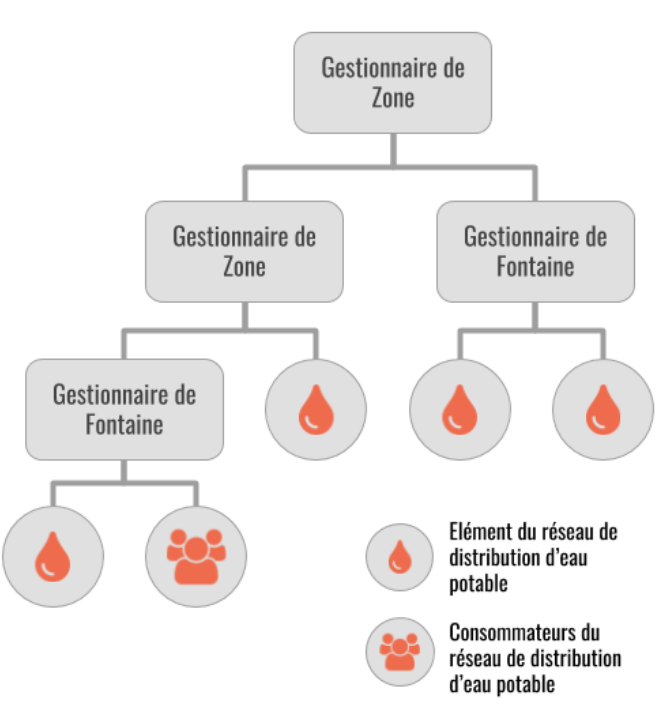
\includegraphics[width=0.5\textwidth]{images/hierarchie}
					\caption{Module consommateurs}
				\end{figure}
				
				
			\subsection{Eléments de l'application}
				\begin{description}
					\item[Zone] Une zone représente une partie du territoire. Une zone peut être subdivisée en plusieurs sous-zone, la zone-parent reprendra alors toutes les données des zones enfants. Cela permet de séparer les responsabilités des différents territoires.
					\item[Elements du réseau] Ces éléments représentent les points physiques du réseau de distribution d'eau potable. Ces éléments sont au nombre de 6 : conduites, réservoirs, sources, fontaines, kiosques et prises individuelles. Tous ensembles ils forment le réseau de distribution au complet. 
					\item[Consommateurs] Le consommateur est une personne qui va utiliser le réseau de distribution d'eau potable. Chaque consommateur se voit lors de son enregistrement attribué à un seul élément de sortie d'eau du réseau : fontaine, kiosque, prise individuelle. De cette façon, il est plus simple de gérer la facturation des consommateurs.
				\end{description}
				
			
				
				%Inclusion du schéma zones, fontaines, ... pour rendre la suite plus claire.
				
			\subsection{Utilisateurs de l'application}
				Il y 2 types d'utilisateurs qui peuvent se connecter à l'application
				
				\begin{description}
					\item[Gestionnaire de fontaine] Ce gestionnaire va gérer la distribution de l'eau aux différents consommateurs. Il devra gérer tous les éléments du réseau qui lui sont attribués.
					\item[Gestionnaire de zone] Ce gestionnaire va avoir la responsabilité de gérer d'autres gestionnaires de zones et/ou des gestionnaires de fontaines. Son travail est plus d'administrer et de surveiller les personnes qui sont en-dessous de lui.			 
				\end{description}
				
				Ces deux gestionnaires vont avoir des privilèges différents et peuvent donc interagir différemment sur les données. Pour illustrer plus simplement cela, voici un tableau tel que présenté ici \cite{ref:haitiwater} où vous pourrez retrouver plus d'informations sur les rôles des différents gestionnaires. 
				\begin{table}[H]
					\centering
					\small
					\setlength\tabcolsep{2pt}
					\begin{tabular}{|l|c|c|}
						\hline
						\multirow{2}{*}{\textbf{Permission}} & \multicolumn{2}{l|}{\textbf{Gestionnaire de}} \\ \cline{2-3}
						 & \textbf{fontaine} & \textbf{zone} \\ \hline
						 Ajouter/modifier/supprimer un consommateur & \cmark & \cmark \\ \hline
						 Ajouter/modifier/supprimer un élément du réseau de distribution & \cmark & \cmark \\ \hline
						 Ajouter/modifier/supprimer un rapport mensuel & \cmark & \cmark \\ \hline
						 Ajouter/modifier/supprimer un paiement & \cmark & \cmark \\ \hline
						 Ajouter/modifier/supprimer un ticket de support & \cmark & \cmark \\ \hline
						 Ajouter/modifier/supprimer une zone & \xmark & \cmark \\ \hline
						 Ajouter/modifier/supprimer un gestionnaire & \xmark & \cmark$^{*}$ \\ \hline
						 Accepter/refuser un changement dans l'historique & \xmark & \cmark \\ \hline
						 \multicolumn{3}{p{\textwidth}}{\emph{* : Un gestionnaire de zone ne peut pas modifier les informations personnelles (mot de passe, courrier, nom, prénom) d'un gestionnaire existant}} \\
					\end{tabular}
					\caption{Permissions dans l'application, par type d'utilisateur}
					\label{tab:permissions}
				\end{table}
				
			\subsection{Accueil}
				Ce module contient les informations condensées de la zone qui est attribuée à l'utilisateur. Il peut y retrouver le nombre de fontaines, de kiosques, de points de prises individuelles et de conduites que contient sa zone mais aussi le nombre de foyers et de consommateurs individuels liés à celle-ci. 
								
				\begin{figure}[H]
					\centering
					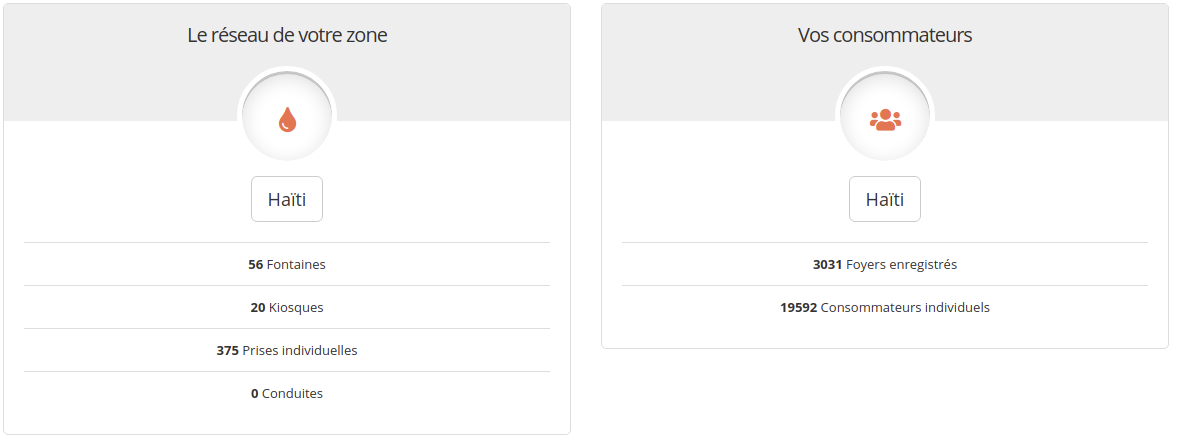
\includegraphics[width=1\textwidth]{images/dashboard}
					\caption{Module d'accueil}
				\end{figure}
				
				
			\subsection{Réseau}
				\label{sec:reseau}
				Dans ce module, l'utilisateur peut retrouver 3 éléments différents.
				
				\begin{description}
				\item[Schéma] Un schéma contenant la répartition des consommateurs par genre ou le volume d'eau mensuel distribué dans chaque zone. Il peut sélectionner le schéma à afficher grâce à une liste déroulante.
				\item[Résumé de zone] Un résumé de sa zone géographique contenant le nombre de consommateurs et de points d'eau présents ainsi que le volume d'eau distribué dans celle-ci.
				\item[Elements du réseau] Un tableau interactif qui contient tous les différents éléments du réseau. Dans cette partie en fonction de ses privilèges, celui-ci peut supprimer, modifier ou ajouter des éléments du réseau. Il peut également trier ou faire des recherches dans ce tableau selon ses besoins.
				\end{description}
				
				\begin{figure}[H]
					\centering
					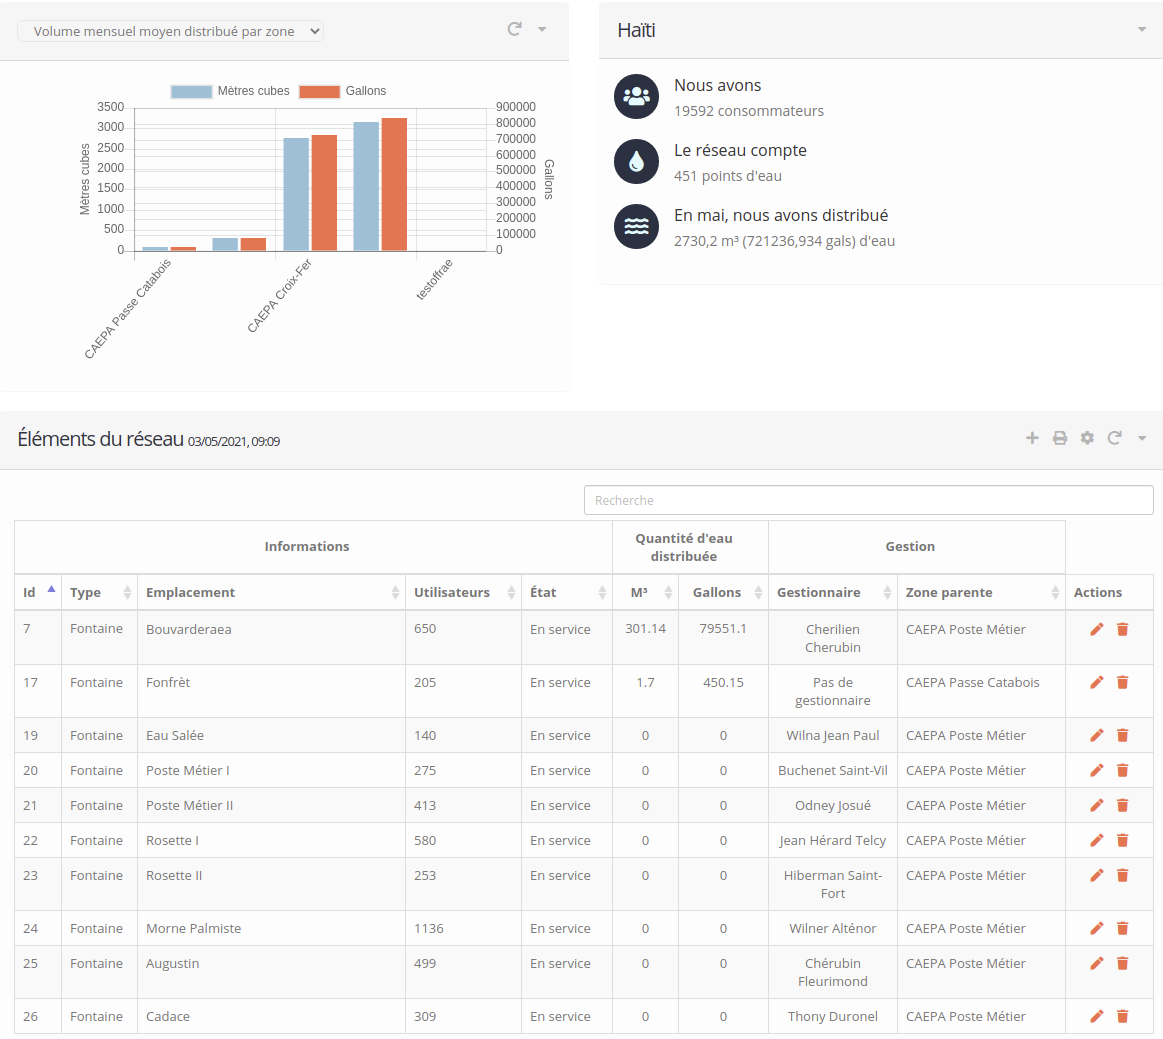
\includegraphics[width=1\textwidth]{images/water_elem}
					\caption{Module réseau}
				\end{figure}
				
\newpage
				
			\subsection{Carte}
				Ce module comprend un tableau réduit des éléments du réseau ainsi qu'une carte interactive qui permet à l'utilisateur de voir où sont situés les différents éléments du réseau et de connaître ou d'encoder les coordonnées géographiques de ceux-ci. 
				
				Comme dans le module \ref{sec:reseau} "Réseau", il est également possible d'ajouter, modifier ou supprimer des éléments du réseau. De plus c'est ici que l'on peut ajouter des coordonnées géographiques à un élément du réseau. Soit en les entrant manuellement soit en utilisant la carte interactive.
				\begin{figure}[H]
					\centering
					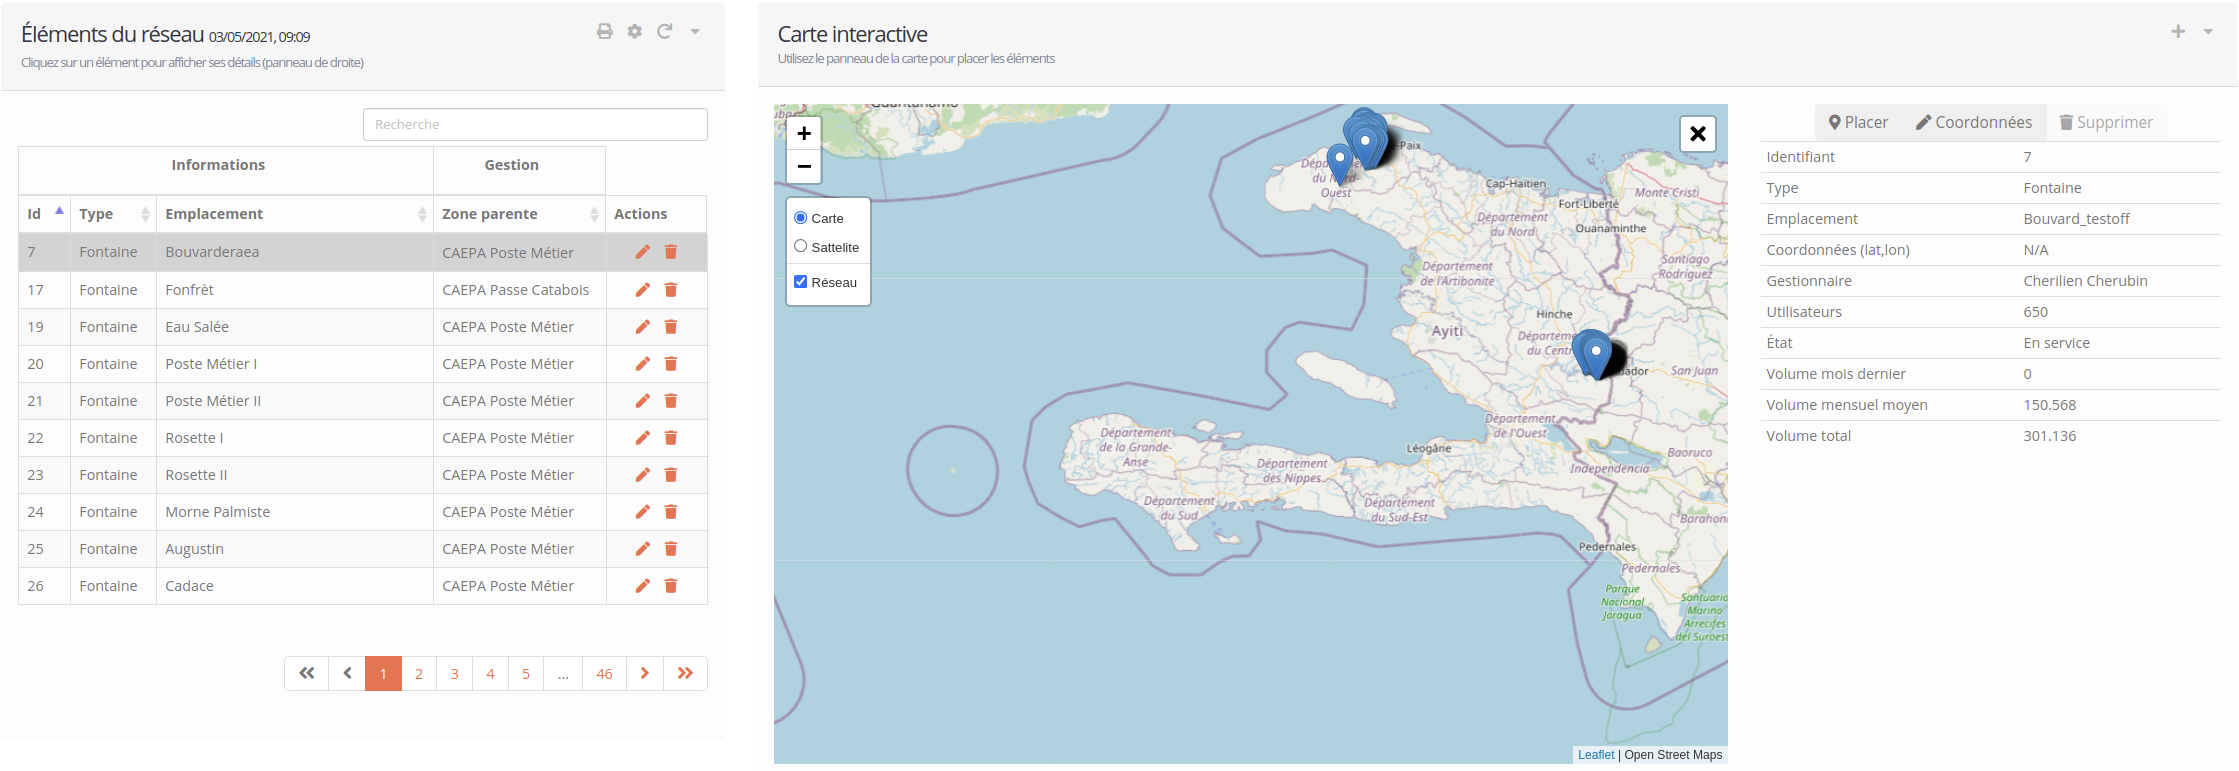
\includegraphics[width=1\textwidth]{images/map}
					\caption{Mordule carte}
				\end{figure}
				
				\begin{figure}[H]
					\begin{subfigure}[b]{0.5\textwidth}
  						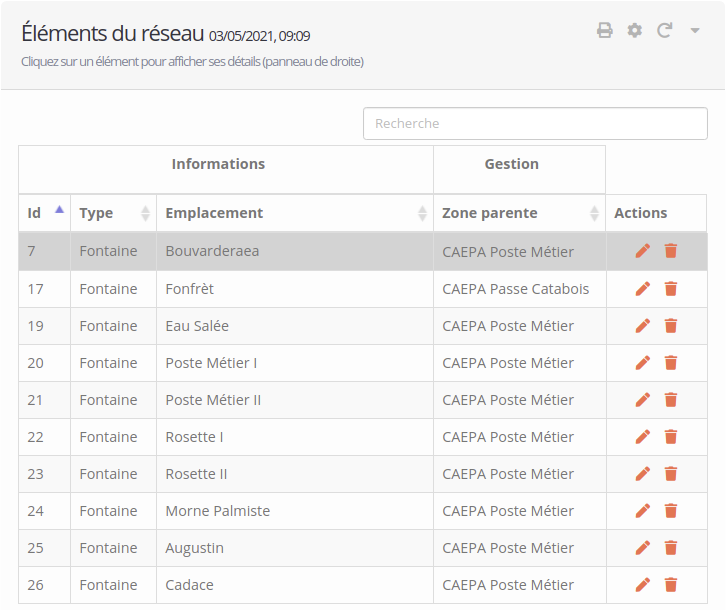
\includegraphics[width=1\linewidth]{images/map_tab1}
  						\caption{Tableau des éléments réseaux simplifié}
					\end{subfigure}%
					\begin{subfigure}[b]{0.5\textwidth}
  						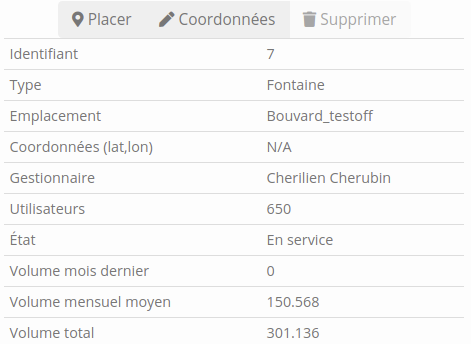
\includegraphics[width=1\linewidth]{images/map_tab2}
  						\caption{Détails de l'élément réseau}
					\end{subfigure}
					\label{fig:test}
				\end{figure}
				
			\subsection{Gestion de zone}
				Ce module comprend 3 tableaux permettant à l'utilisateur de gérer sa zone.
				\begin{description}
					\item[Zones] Le premier contient les différentes zones géographiques encodées dans le système. Cliquer sur un des éléments du tableau permet de filtrer les éléments des deux autres tableaux qui seront décrits plus bas afin de ne garder que les éléments de la zone concernée. Ce tableau permet également si l'utilisateur a les privilèges requis d'ajouter, supprimer ou modifier une zone.
					\item[Gestionnaires] Le deuxième contient la liste de tous les gestionnaires. Cliquer sur un gestionnaire permet à l'utilisateur de filtrer les éléments réseaux qui sont gérés par ce gestionnaire. De nouveau si l'utilisateur possède les privilèges nécessaires, il pourra ajouter, modifier ou supprimer des gestionnaires.
					\item [Elements du réseau] Le dernier contient le même tableau que dans la section \ref{sec:reseau} "Réseau".
				\end{description}
				\begin{figure}[H]
					\centering
					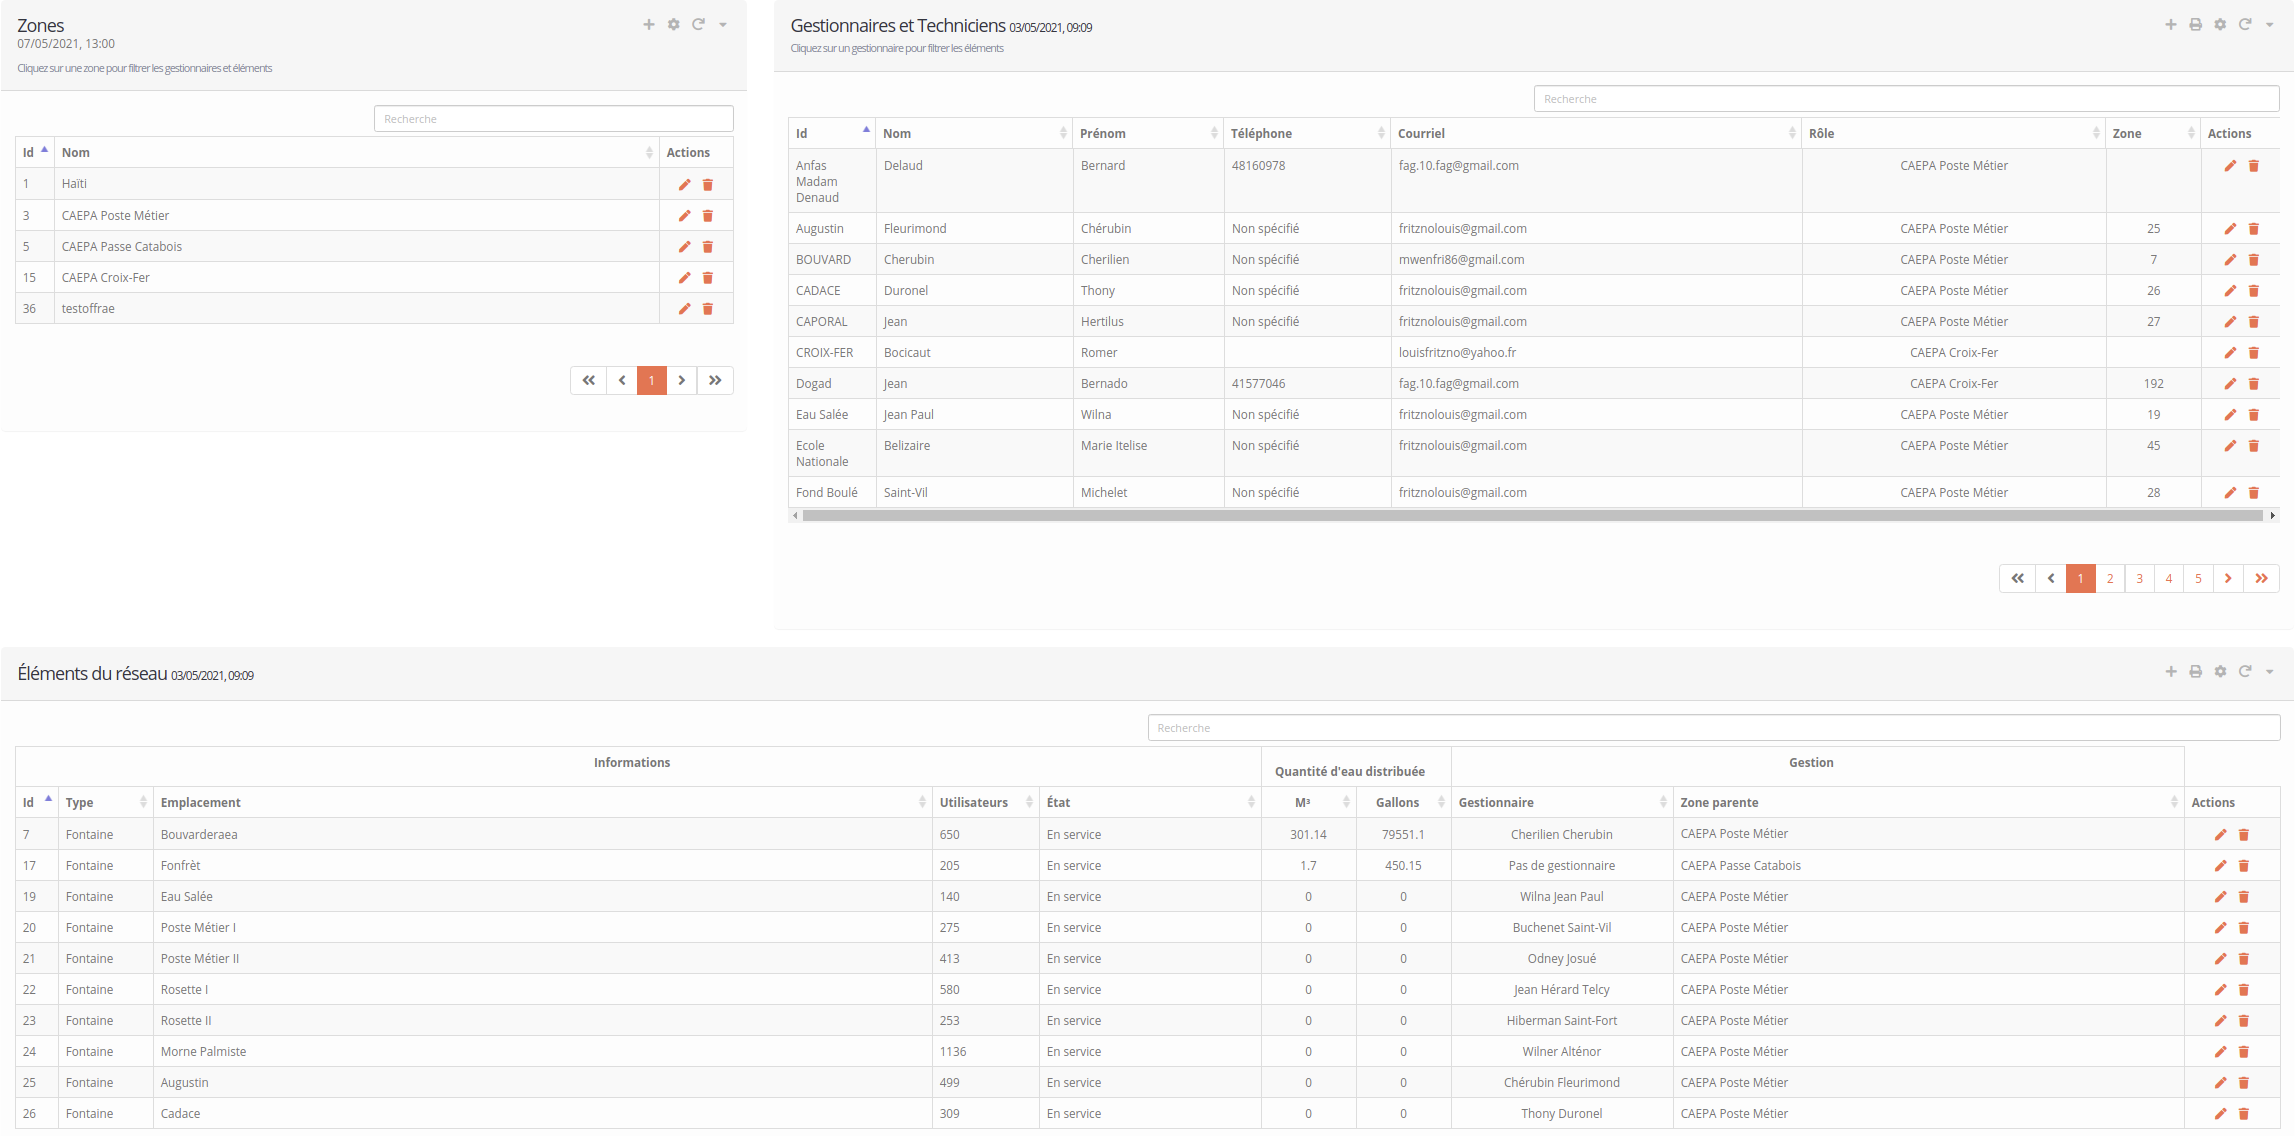
\includegraphics[width=1\textwidth]{images/gestion}
					\caption{Module gestion de zone}
				\end{figure}
			
				
				\begin{figure}[H]
					\begin{subfigure}[b]{0.3\textwidth}
  						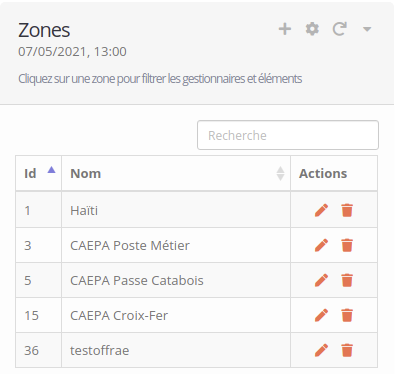
\includegraphics[width=1\linewidth]{images/gestion_tab1}
  						\caption{Tableau des zones}
					\end{subfigure}%
					\begin{subfigure}[b]{0.7\textwidth}
  						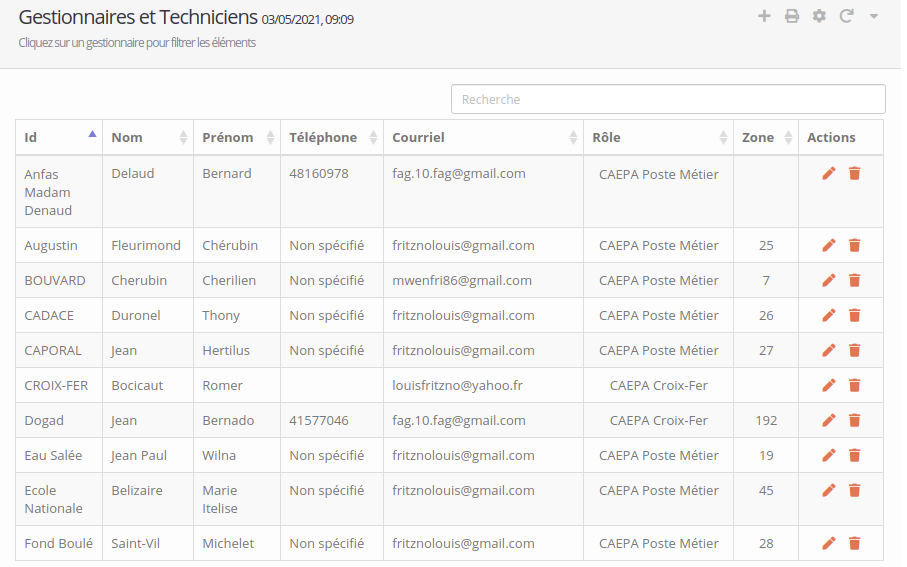
\includegraphics[width=1\linewidth]{images/gestion_tab2}
  						\caption{Tableau des gestionnaires}
					\end{subfigure}
					\label{fig:test}
				\end{figure}
			
			\subsection{Historique}
				Ce module contient les actions ayant été effectuées par des gestionnaires de fontaines. Ces actions doivent être validées ou refusées par un gestionnaire plus haut placé. On peut y retrouver deux tableaux.
				\begin{description}
					\item[A valider] Le tableau du haut contient les éléments devant être validés. Ici si l'utilisateur a les privilèges requis, il peut choisir de confirmer ou non une action qui a été encodée.
					\item[Historique] Le tableau du bas contient les éléments qui ont été validés ou refusés dans les 3 dernières semaines. Il s'agit simplement d'un historique récent.
				\end{description}
				\begin{figure}[H]
					\centering
					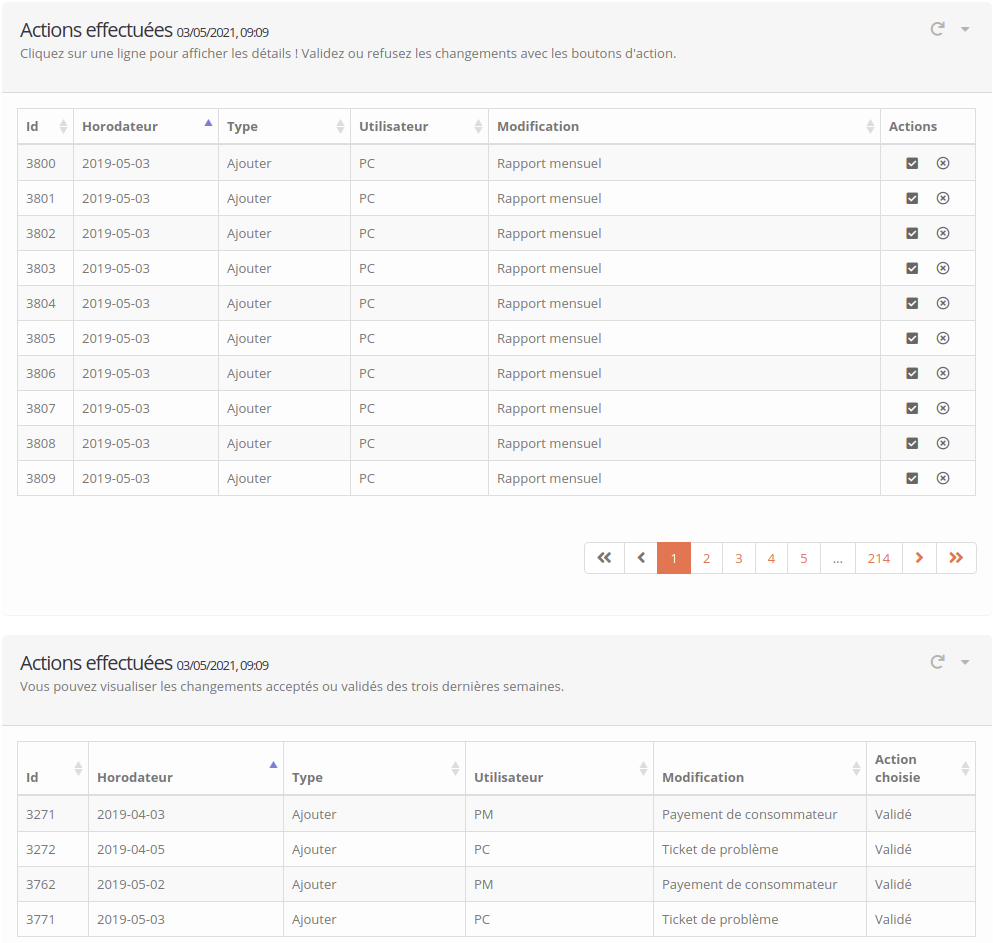
\includegraphics[width=1\textwidth]{images/logs}
					\caption{Module historique}
				\end{figure}
			
			\subsection{Rapports}
				Dans ce module, l'utilisateur peut signaler les différents problèmes qu'il rencontre avec les infrastructures de distribution d'eau. Une fois le problème signalé, celui-ci peut consulter ce qu'il a encodé dans le tableau juste en dessous et modifier ou supprimer son signalement. Si ses privilèges sont suffisamment élevés, il pourra également gérer les signalements des autres personnes.
				
				C'est également ici que l'utilisateur va pouvoir encoder les rapports mensuels. Si jamais la connexion internet n'est plus présente, il peut simplement enregistrer le formulaire avec les données qu'il a encodés afin de l'envoyer plus tard lorsque le réseau sera de nouveau accessible.
				
				\begin{figure}[H]
					\centering
					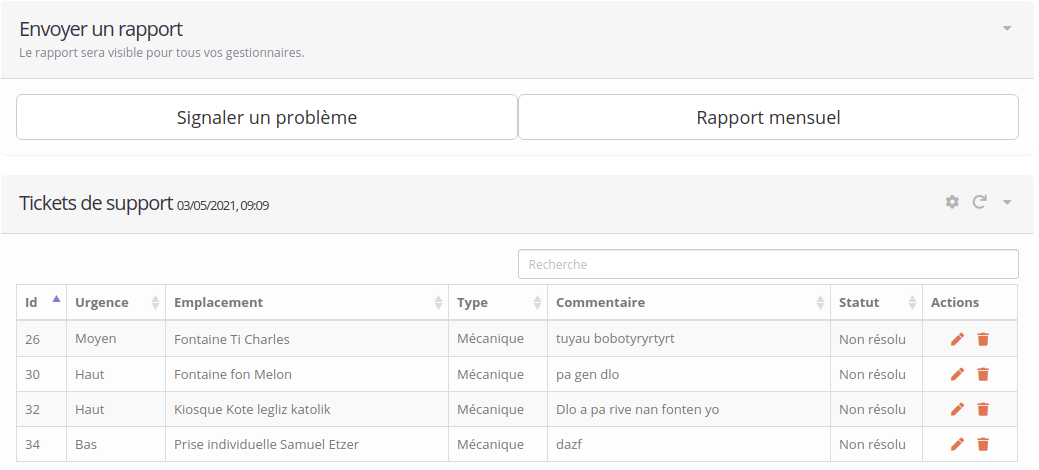
\includegraphics[width=1\textwidth]{images/report}
					\caption{Module rapport}
				\end{figure}
			
			\subsection{Consommateurs}
				Dans ce module, l'utilisateur retrouve 3 parties différentes :
				\begin{description}
					\item[Schéma] Le même choix de schéma que décrit dans la section \ref{sec:reseau}.
					\item[Résumé de zone] Un résumé de la situation de votre zone (nombre de foyers consommant de l'eau, nombre de consommateurs, nombre de foyers n'ayant pas payé leur facture).
					\item[Consommateurs] Un tableau qui reprend tous les consommateurs auxquels l'utilisateur a accès. Celui-ci peut ajouter, modifier ou supprimer des consommateurs. Ou bien il peut également juste consulter tous les détails sur ceux-ci.
				\end{description}

				
				\begin{figure}[H]
					\centering
					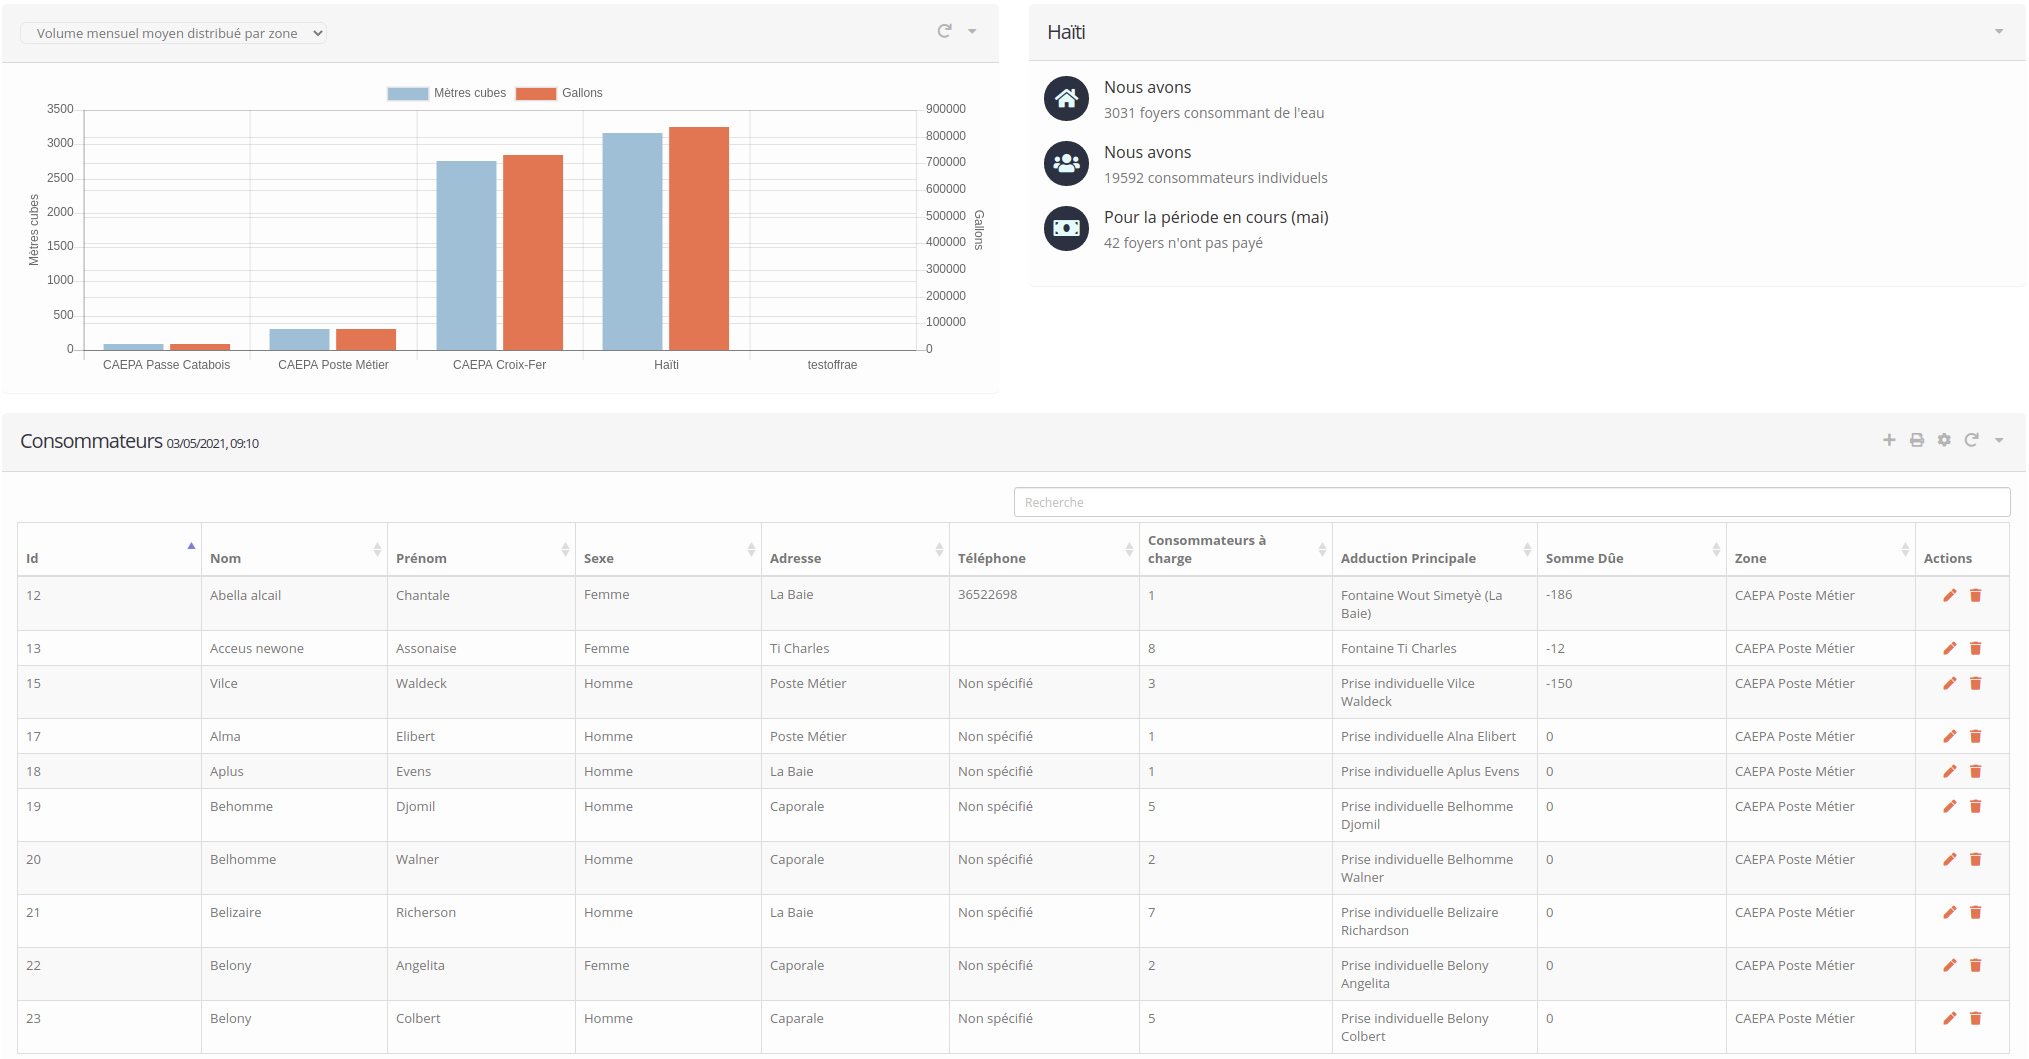
\includegraphics[width=1\textwidth]{images/consumer}
					\caption{Module consommateurs}
				\end{figure}
				
				\begin{figure}[H]
					\centering
					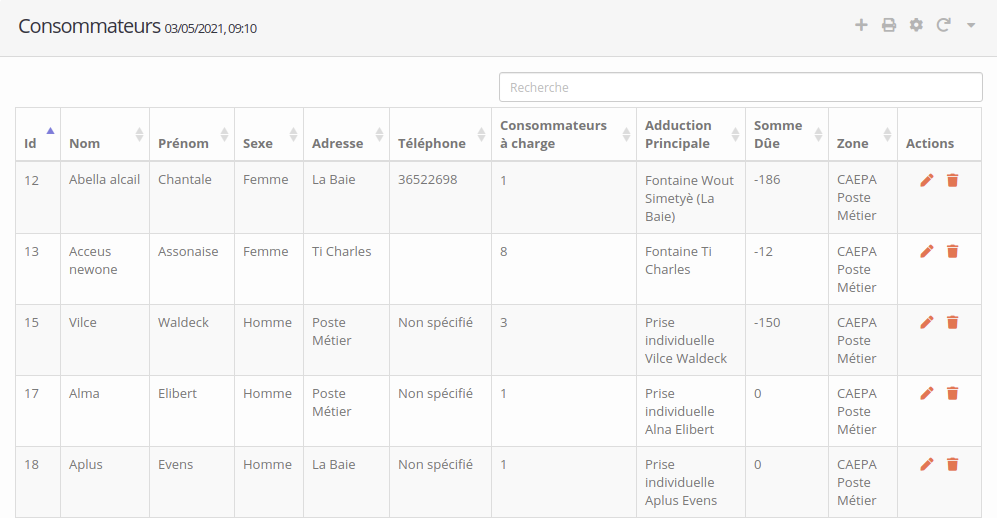
\includegraphics[width=1\textwidth]{images/consumer_tab1}
					\caption{Tableau des consommateurs}
				\end{figure}
			
\newpage
			\subsection{Finances}
				Dans ce module, l'utilisateur a accès à 4 tableaux différents qui lui permettent de gérer les finances de ses consommateurs. Celui-ci pourra modifier, supprimer ou ajouter des informations dans les différents tableaux en fonction de son niveau de privilèges.
				\begin{description}
					\item[Zones] Un tableau contenant les différentes zones. Le fait de sélectionner une zone permet à l'utilisateur de filtrer les consommateurs en fonction de leur zone d'attribution.
					\item[Consommateurs] Un tableau contenant les consommateurs auxquels l'utilisateur a accès. Le fait de sélectionner un consommateur permet de faire apparaître les deux tableaux suivants.
					\item[Détails] Un tableau contenant les coordonnées du consommateur sélectionné ainsi que la somme due par celui-ci. Il n'est pas possible de modifier des données manuellement dans ce tableau.
					\item[Paiements] Un tableau interactif contenant tous les paiements effectués par le consommateur sélectionné. Ici l'utilisateur peut ajouter, modifier ou supprimer des paiements.
				\end{description}
				
				\begin{figure}[H]
					\centering
					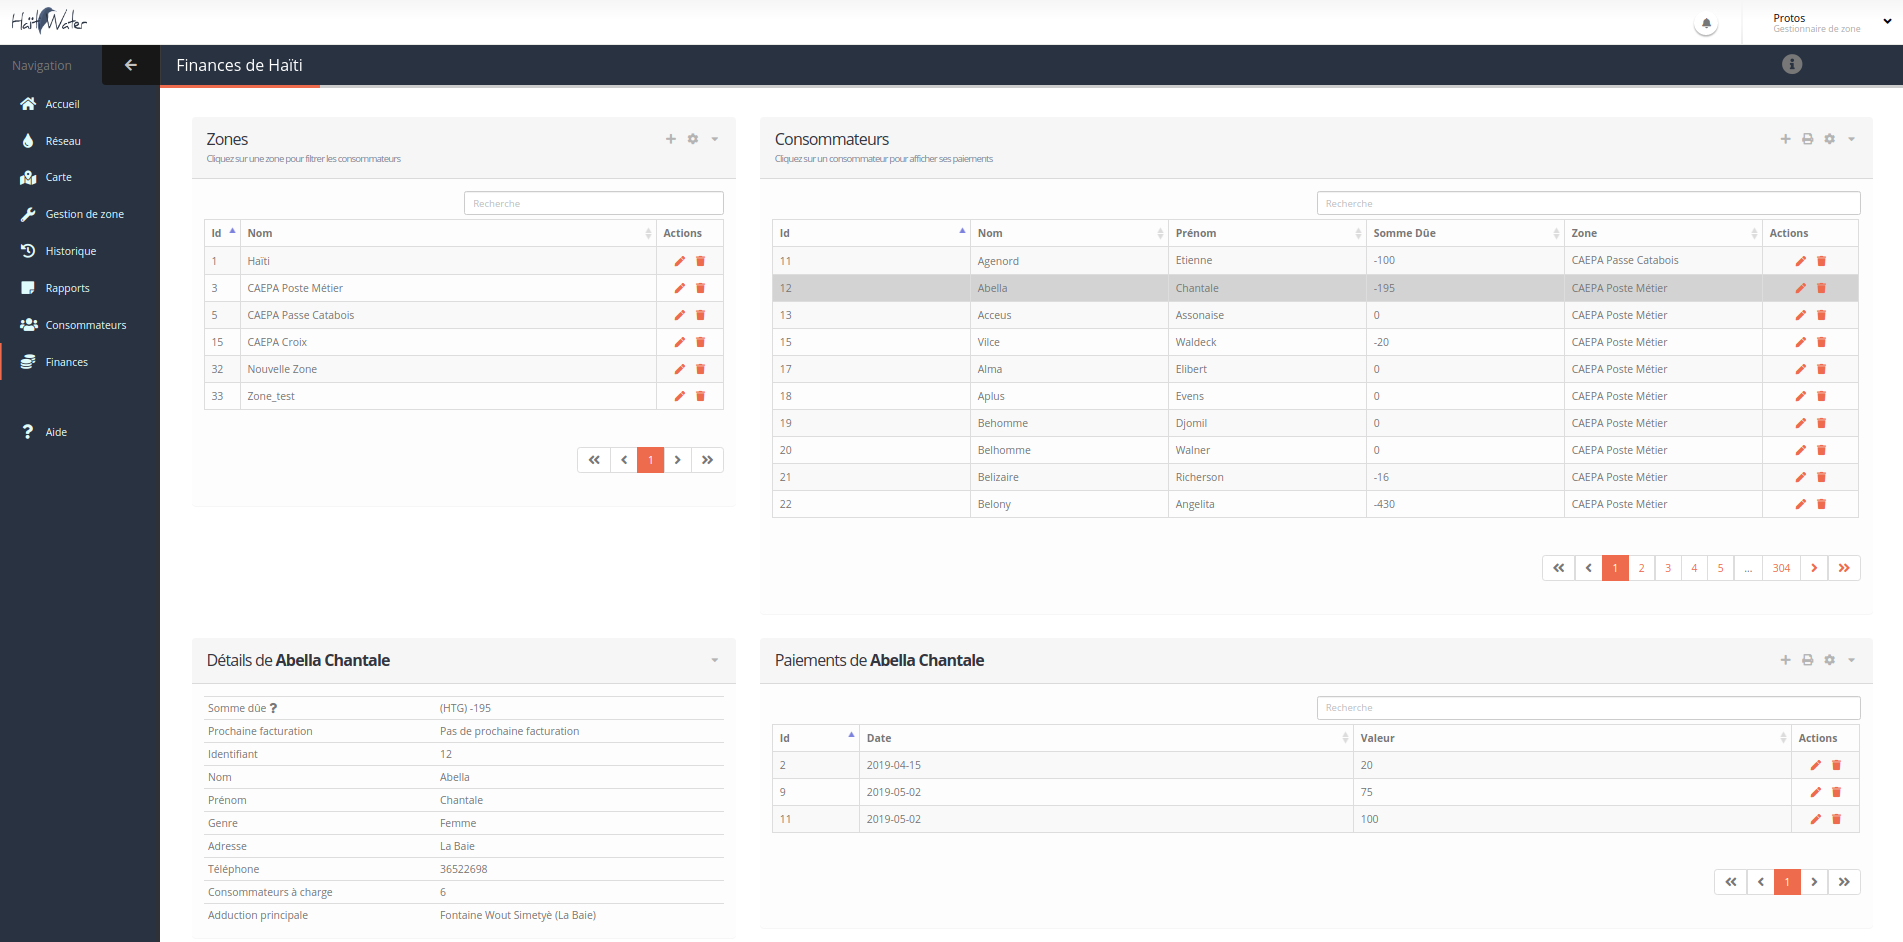
\includegraphics[width=1\textwidth]{images/finances}
					\caption{Module finances}
				\end{figure}
				
				
		\section{Problèmes réseaux}
			L'application HaïtiWater est une application web classique. Cela signifie que pour fonctionner, il faut qu'il y ait nécessairement une connexion à internet. Or en Haïti, cette connexion n'est pas très stable en ville et celui-ci peut aller jusqu'à être inexistant lorsque vous vous aventurez dans les zones les plus rurales. 
			
			Ces problèmes de connexions font que l'application est difficilement utilisable sur le terrain en toute sérénité car on ne sait jamais quand le réseau va devenir capricieux. Pour pallier ce problème, il a été décidé de transformer l'application web existante pour que celle-ci puisse fonctionner même lorsque le réseau est absent.
				
			De par sa nature, une application web nécessite un connexion pour pouvoir fonctionner. Il a donc fallu étudier les différentes options qui pourraient permettre de faire fonctionner l'application hors-ligne. Parmis les ces options,  les deux qui ont été retenues étaient de soit créer une \textbf{application mobile} séparée de l'application web, soit de transformer l'application web existante en \textbf{Progressive Web App}. 
				
			L'avantage de créer une application dédiée aux mobiles est qu'il est très simple de gérer le fonctionnement hors-ligne de cette application. De plus on peut plus facilement utiliser les différentes capacités de l'appareil mobile comme la caméra, la localisation, ...
			L'inconvénient de cette solution est qu'il fallait du coup générer une nouvelle application de A à Z. De plus cela implique qu'il y aura deux codes différents dans deux langages différents à devoir maintenir.
				
			L'avantage de la Progressive Web App est que tout se joue au niveau du navigateur. Il n'est donc pas nécessaire de devoir maintenir un deuxième code source. De plus aucune installation n'est nécessaire de la part de l'utilisateur et les mises à jour de l'application sont faites de manière transparente.
			L'inconvénient de cette solution est que la gestion du mode hors-ligne est un peu plus complexe, on ne peut pas profiter des capacités de l'appareil mobile aussi bien qu'avec une application native et cette technologie étant assez récente, il n'y a pas énormément de ressource d'aide en ligne et tous les navigateurs ne prennent pas en charge toutes les fonctionnalités proposées.
				
			Au vu de la situation compliquée en Haïti et du temps qui sera alloué à ce mémoire, il a été décidé que la meilleure option était celle de la Progressive Web-App. La raison principale est qu'il aurait difficile une fois le mémoire terminé d'avoir deux codes sources différents à maintenir et à mettre à jour.
			
			
			
			
%------------------------------------------------------------------------------------------

	\chapter{Organisation}
		Étant le seul étudiant à réaliser ce mémoire, il n'a pas été nécessaire d'utiliser des outils de planification complets. Cette section contiendra surtout la planification des différentes tâches à accomplir permettant l'aboutissement de l'application ainsi que l'écriture de ce mémoire. Celles-ci ont été mises en place grâce aux discussions avec mes deux promoteurs. 

		\section{Approche de travail}
			La première étape du mémoire a été de bien mettre en avant les différentes fonctionnalités à implémenter afin d'ajouter de la plus value au projet existant. L'idée de base étant de rendre l'application fonctionnelle hors-connexion.	
			
			Nous avons étudié la question avec mes deux promoteurs et Nahomie, l'étudiante venue d'Haïti. Celle-ci à pu nous apporter son expertise afin de séléctionner les fonctionnalités qui pourraient apporter une réelle valeur au projet et prioriser l'implémentation de celles-ci.
		
			%Comprendre les enjeux et les différentes problématiques a été la première tâche à accomplir. Il a fallut décider du type de technologie à utiliser afin d'apporter les fonctionnalités nécessaires au bon fonctionnement de l'application. 
			
			%La meilleure option aurait été de pouvoir en discuter avec la plupart des acteurs en Haïti afin d'avoir le plus d'avis possible sur la question. Mais vu le temps que cela aurait pris cette option n'était pas du tout envisageable. Pour pallier à se problème, nous avons étudié la question avec mes deux promoteurs et Nahomie l'étudiante venue d'Haïti. Celle-ci à pu nous apporter son expertise afin de choisir l'option idéale.
			
			%Une fois le choix technologique fait, nous avons effectuer la planification des tâches.
		
		

			%Etude du problème
			%Prioritisation des taches

			\subsection*{Planification}
				\label{sec:planification}
				
				\paragraph*{Mensuel}
				Dans un premier temps, il a fallu réaliser un plan général de déroulement du mémoire et mettre en avant les modules sur lesquels il fallait travailler en priorité et les différentes fonctionnalités à implémenter dans ceux-ci. Une grosse échéance était de pouvoir faire tester l'application par de vraie personne à partir de Février afin d'obtenir du feedback sur l'application.
				
				%Malgrè tout il était difficile de mettre des dates fixes car la technologie utilisée comporte encore peu de communauté et il est donc difficile de trouver des solutions "clé sur porte". 
				%La grande échéance posée était de pouvoir effectuer les tests de l'application avec des personnes réelles à partir de février afin d'avoir le temps de prendre compte les feedback pour améliorer l'application.
				
				\paragraph*{Hebdomadaire} 
				Une réunion était prévue toutes les semaines en alternance avec mes deux promoteurs. Ces réunions permettaient de leur montrer l'état d'avancement du développement et d'avoir un feedback extérieur sur celui-ci. 
				Ces réunions ont toutes eu lieu en vocal via l'application Teams. En effet en période de COVID, il était impossible de se voir régulièrement en présentiel.
				
				\paragraph*{Quotidien}
				Etant donné que j'étais le seul à travailler sur le mémoire, un outil de suivi n'était pas nécessaire. Pour gérer l'organisation du travail une simple liste de tâches était maintenue. Cette liste était modifiée tous les jours en fonction de l'avancement de celles-ci. Les plus importantes étaient maintenues en haut de la liste afin de les prioriser. 
				
				Le plan n'a malheureusement pas pu être entièrement respecté pour différentes raisons:
				\begin{itemize}
					\item La technologie étant encore assez récente, les sources d'informations et d'aides sur le net sont encore peu présente. Du retard a donc été pris lors du développement de certaines fonctionnalités complexes.
					\item L'installation du serveur en Haïti a pris plus de temps que prévu et il a donc fallu repousser la validation avec de vraies personnes. 
					\item La période COVID-19 a apporté un manque de stimulation et de motivation qui a ralenti l'avancement du projet.
				
				\end{itemize}				
				
				Malgrè le retard pris, il a tout de même été possible de terminer le projet dans les temps.
				
				
		\section{Méthodologie}
			Même en travaillant seul, une bonne méthodologie de travail permet de garantir l'avancement régulier du projet. Elle permettra de transformer efficacement les différents besoins en fonctionnalités implémentées.
			

			\subsection*{Agile}
				Le méthodologie agile permet une réponse au changement plus flexible. Plûtot que de planifier tout le projet directement, on développe par petit incrément que l'on termine termine à chaque itération. 
				
				Cette méthode a permis de faire évoluer le projet en fonction des différents feedback reçu par les promoteurs et par l'étudiante venue d'Haïti. Ce qui n'aurait pas été possible avec une approche waterfall beaucoup plus séquentielle.
				
				\paragraph*{Feature Driven Development.} L'application a été développée avec la méthode de développement par les fonctionnalités. Dans cette méthode on se focalise surtout sur la création d'une liste de fonctionnalités et sur leurs productions. Les différentes fonctionnalités ont été déterminées par mes deux promoteurs et l'étudiante de Haïti.
				
				\paragraph*{Itérations} Dans le cadre d'une méthodologie agile, les itérations sont de courtes durées. Lors de ce mémoire, les itérations duraient deux semaines. Cela permettait d'avoir un feedback de la part des deux promoteurs que je voyaient en alternance une semaine sur deux.
				Les avantages des itérations courtes sont que l'on peut détecter rapidement les défauts présents et de les corriger. 


			\subsection*{Phases du mémoire}
				%Le développement des nouvelles fonctionnalités de l'application c'est fait de manière agile et est donc surtout composée de beaucoup de petites phases. Par contre, pour ce qui est du déroulement du mémoire en lui-même, il y a différentes grandes phases qui se sont dessinées.
			%Les raisons à cela sont que certaines phases n'étaient pas réalisable avant que d'autres ne soit complètement terminées ou presque. 
			
			\begin{figure}[H]
					\centering
					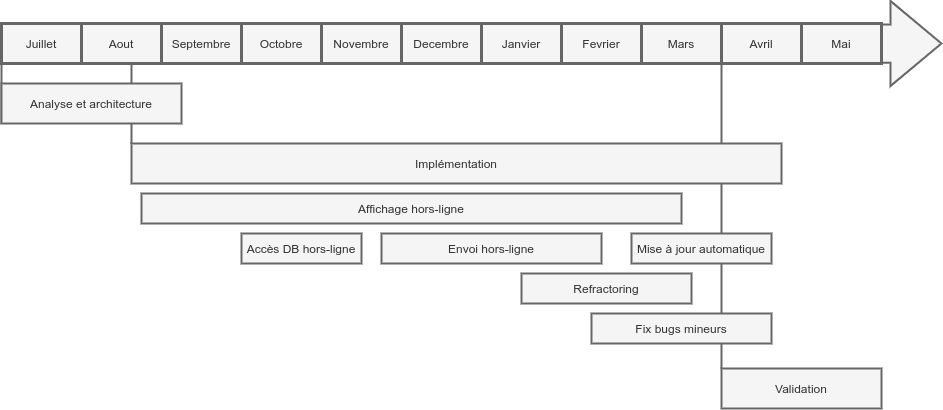
\includegraphics[width=1\textwidth]{images/Gantt}
					\caption{Diagramme de Gantt}
					\label{fig:Gantt}
				\end{figure}
				
			\paragraph*{Analyse et architecture.}
			Sur le schéma \ref{fig:Gantt}, on peut voir qu'il y a d'abord une phase d'analyse afin de déterminer les technologies qui seraient utilisées pour les différentes fonctions à implémenter. C'est dans cette phase qu'il y a eu beaucoup de discussions avec l'étudiante venue d'Haïti.
		
			\paragraph*{Implémentation.} 
			Cette phase compose la plus grosse partie du mémoire. C'est ici que toutes les décisions prises durant la phase d'analyse se sont mise en place. Cette phase se divise en plusieurs petites phases qui représentent les différentes fonctionnalités produites durant le mémoire. 
			
			\paragraph*{Validation.}
			La phase de validation n'intervient que tard dans le déroulement du mémoire. C'est simplement parce que la méconnaissance de la technologie à utiliser et le temps qu'a pris le déploiement de l'application sur les serveurs Haïtiens ont grandement retardé l'arrivée de cette phase.			
			
			\paragraph*{Rédaction.}
			La rédaction du mémoire n'a commencé que lorsque la plupart des fonctionnalités étaient terminées afin de lancer la validation au plus vite. Durant la rédaction, les parties produites ont été relues par mes deux promoteurs séparément afin d'améliorer celle-ci mais aussi par des relecteurs externes afin que le texte soit plus agréable à lire. 
			
			
			
			
			
%---------------------------------------------------------------------------------------------

	\chapter{Analyse des besoins}
		\label{sec:analyse_besoins}
		Cette phase est très importante. C'est lors de celle-ci que nous, mes deux promoteurs, l'étudiante d'Haïti et moi-même, avons choisi quelle technologie était la plus adaptée afin de faire évoluer l'application existante de la meilleure façon possible. C'est également ici qu'on été déterminé toutes les fonctionnalités à implémenter et leur ordre de priorité.
		
		J'ai avec l'aide de l'étudiante Haïtienne et les bons conseils de mes promoteurs, realiser une analyse de MoSCoW qui sera décrite dans la section \ref{sec:besoins_fonctionnels}. Cette méthode permet de prioriser les tâches d'un projet en fonction de leur criticité, c'est-à-dire du niveau d'impact de la tâche sur la réalisation du projet.
		
		Cette analyse de moscow est assez représentative de la direction que devait prendre le projet et représente bien les différentes tâches à accomplir. En accord avec cette analyse, toutes les taĉhes de type \textbf{M}, \textbf{S} et \textbf{C} ont été réalisée durant ce projet. Seule les tâches \textbf{W} n'ont pas été implémentées.


		\section{Besoins fonctionnels}
			\label{sec:besoins_fonctionnels}	
				
			\begin{figure}[H]
				\centering
				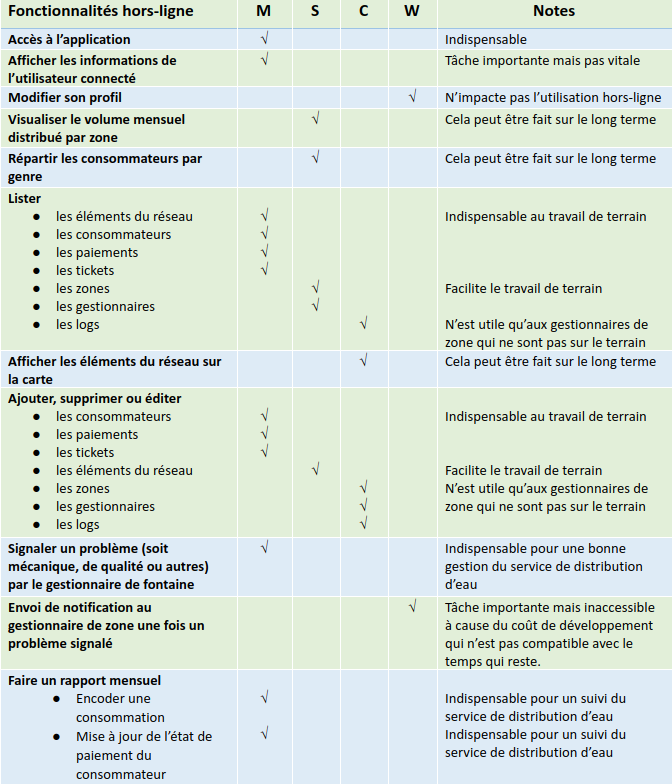
\includegraphics[width=1\textwidth]{images/moscow}
				\caption{MoSCoW}
			\end{figure}
			
			Les besoins fonctionnels répondent aux points précis à implémenter, ils représentent toutes les tâches à accomplir pour que le projet soit réussi.

			Dans le tableau de MoSCoW, les lettres ont le signification suivante: 
			\begin{description}
				\item[M] signifie "Must have", le projet serait un échec si l'application ne possèdait pas cette fonctionnalité à la fin du développement.
				\item[S] signifie "Should have", cette fonctionnalité doit être faite dans la mesure du possible. Ces tâches sont importantes mais pas vitales.
				\item[C] signifie "Could have", cette fonctionnalité peut être faite si cela n'affecte pas les autres tâches importantes. Ce sont des tâches de confort qui peuvent être effectuées si vous avez suffisamment de temps et que les tâches des deux catégories précédentes ont été réalisées.
				\item[W] signifie "Won't have but would like", ce qui ne sera pas fait cette fois, mais plus tard. Réaliser ces tâches est un luxe qu'on a théoriquement pas le temps de se payer.
			\end{description}
			
			Lors de l'analyse des besoins, non avons bien entendu repris l'analyse faite ici \cite{ref:haitiwater}. Les 3 options proposées sont les suivantes. 
			\begin{description}
				\item[Simple formulaire.] Cette solution consiste a faire en sorte que l'on puisse enregistrer les différents formulaires lorsque le réseau n'est pas disponible à la manière de ce qui exite déjà dans l'application pour l'ajout d'un rapport mensuel. C'est la solution la plus simple car elle ne demande pas d'avoir les données de la base synchronisée localement. Pourtant cette solution n'a pas été retenue car celle-ci est trop simpliste et ne permet pas une utilisation suffisante en cas de perte de connexion.
				\item[Accès statique.] Cette solution demande d'avoir une version simplifiée de la base de données en copie sur l'appareil de l'utilisateur mais sans la possibilité de modifier celle-ci. Cela permettrait aux utilisateurs de consulter les données hors-ligne mais pas d'en entrer de nouvelles. L'avantage de cette solution est que la synchronisation des tâbles est très simple et qu'il n'y a pas de problèmes d'inconsistances des données.
				\item[Accès complet.] Cette solution permettrait aux utilisateurs de pouvoir consulter, ajouter, supprimer et modifier des données de la base de données. Ainsi même en cas de perte de réseau, l'utilisateur pourrait continuer à réaliser ses tâches sans le moindre soucis. Cette solution est la plus compliquée à mettre en place car elle demande de synchroniser les différentes versions des données. En effet si deux utilisateurs modifient en même temps les mêmes données en étant hors-ligne, il faudrait pouvoir déterminer quelle modification conserver sans créer d'inconsistances.  
			\end{description}
			
			L'option qui a été choisie est celle de l'accès complet. C'est la seule solution qui permettrait vraiment à l'application d'être utilisée de manière intensive sur le terrain. C'est également l'option la plus intéressante à mettre en place du point de vue technique.
			
			
			\subsection*{Affichage des pages}
				Une partie importante des besoins est bien évidemment l'accès aux différentes pages de l'application lorsque la connexion internet n'est plus disponible. 
				
				C'était la partie prioritaire du projet car sans cette fonctionnalité, il aurait été impossible d'accèder aux différentes données. Les premières pages concernées par cette évolution ont été celles utiles aux gestionnaires de fontaines qui sont le plus souvent sur le terrain.
				Les différents points du tableau de moscow concerné par cette partie sont :
				\begin{itemize}
					\item L'accès à l'application
					\item Afficher les informations de l'utilisateur connecté
					\item Visualiser le volume mensuel distribué par zone (schéma)
					\item Répartir les consommateurs par genre (schéma)
				\end{itemize}
				
				Comme on peut le voir les deux premiers points sont bien placés dans la catégorie "Must have". Les deux derniers sont dans le "Should have" car ils ne sont que des schémas et pas des pages à part entière.
				
			\subsection*{Accès aux données}
				La deuxième partie importante des besoins fonctionnels est d'avoir accès aux données de la base de données même lorsque la connexion internet n'est pas disponible. En effet le simple accès aux pages hors ligne n'a que peu d'intérêt si l'on ne peut pas consulter de données sur ces pages.
			Dans le tableau de moscow, cela est représenté les points suivants :
				\begin{itemize}
					\item Lister les éléments du réseau
					\item Lister les consommateurs
					\item Lister les paiements
					\item Lister les tickets
					\item Lister les zones
					\item Lister les gestionnaires
					\item Lister les logs
				\end{itemize}
				
				Les quatres premiers points sont dans la catégorie "Must have" car ceux-ci représentent les données qui seront utilisées en permanence par les acteurs sur le terrain, dans notre cas les gestionnaires de fontaines. Ce sont donc les données qu'il faut avoir prioritairement dans l'application hors-ligne.
				
				Les trois derniers sont dans la catégorie "Should have" et "Could have" car ceux-ci sont surtout utile pour les gestionnaires de zones qui seront assez peu sur le terrain. Malgrè tout il reste intéressant de pouvoir accèder à ces données même lorsque le réseau internet n'est pas disponible dans le cas où un gestionnaire devrait se déplacer sur le terrain ou bien en cas de panne réseau.
				
				Un dernier point non listé est d'afficher les éléments du réseau de distribution d'eau sur une carte interactive même lorsque l'on a pas de connexion réseau. Ce point a été mis dans les "Could have" car l'usage de la carte en mode hors-ligne est une fonction qui prendrait beaucoup d'espace sur un appareil mobile et cette fonctionnalité n'est pas essentielle à un usage sur le terrain.

			\subsection*{Modifications des données}
				\label{sec:gest_donnee}
				La dernière partie mais non la moindre consiste à gérer l'envoi des données lorsque la connexion au réseau n'est pas disponible. Cela permettrait aux utilisateurs de pouvoir complétement se passer de la solution crayon/papier.
				Dans le tableau de moscow cette partie est représentée par les points suivant:
				\begin{itemize}
					\item Ajouter, supprimer ou éditer
					\item Signaler un problème par le gestionnaire de fontaine
					\item Faire un rapport mensuel
				\end{itemize}
				
				La plupart des points sont situés dans la partie "Must have" car ces fonctionnalités sont essentielles au bon fonctionnement de l'application hors-ligne. Par contre la modification des éléments du réseau, des zones, des gestionnaires et des tickets sont dans les catégories "Should have" and "Could have" car ces données sont surtout utilisées par les gesionnaires de zones qui ne vont que peu sur le terrain et pas par les gestionnaires de fontaines.			

		\section{Besoins non-fonctionnels}
			Les besoins non-fonctionnels sont soit des besoins optionnels, soit des besoins liés à l'implémentation et à l'interopérabilité générale. En réalisant ces besoins non fonctionnels, on obtient un système fiable et qualitatif.
					
			\subsection*{Multi-plateforme}
			\label{sec:multi}
				Ce projet se déroule dans le cadre, et est la suite, d'un mémoire universitaire. La prochaine étape pour celui-ci une fois le mémoire terminé est qu'il soit déployé et maintenu par une équipe de développeur en Haïti. 
				
				Le problème est qu'on ne connait pas encore le temps et le budget qui seront alloués à la suite de ce projet. Par contre, ce que l'on sait, c'est qu'il faut que l'application puisse tourner sur un maximum d'appareils différents. Les choix technologiques qui seront décris dans le section \ref{sec:choix_tech} ont donc été pris en prenant en considération le fait que l'application doit pouvoir tourner sur tout type de configuration.
				
			\subsection*{Technologies simples et populaires}
				Comme précisé précédemment, nous ne connaissons pas encore l'équipe de développeur qui va reprendre le projet. Il a donc fallu continuer à utiliser des technologies qui sont assez rapide à apprendre et accessible à tous. Cela afin de faciliter la maintenance et l'évolutivité de l'application lorsque celle-ci sera déployée en Haïti.	
				
		\section{Structure des données hors-ligne}
			\label{sec:data}
			Pour que l'utilisateur puisse accèder aux données en étant hors-ligne, il faut bien évidemment que celles-ci soient stockées sur l'appareil. Pour ce faire il a fallu trouver une solution qui prendrait peu de place sur l'appareil de l'utilisateur, qui permettrait un accès rapide en lecture et la possibilité de modifier ces données. Deux solutions ont alors été envisagées.
			\begin{description}
				\item[JSON] Stocker les réponses au format JSON telles qu'envoyées par le serveur dans la cache du navigateur. L'avantage de cette solution est qu'il est très rapide de récupérer les données à afficher sur la page lors du chargement de celle-ci car les données nécéssaires sont stockées telles quelles dans le navigateur, elle est également très facile à mettre en place. Si l'on avait utilisé l'accès statique aux données comme décrit dans la section \ref{sec:besoins_fonctionnels}, cette solution aurait été suffisante. Mais comme il faut pouvoir modifier les données, cette solution est suboptimal.
				\item[DB] Utiliser un système de gestion des données intégré au navigateur. Cette option a pour avantage le fait d'avoir un vrai système de gestion de données. Une fois les données enregistrées dans le navigateur, il est très facile de faire des requêtes sur ces données ou bien d'ajouter en modifier certaines. Par contre l'inconvénient est que lors de la synchronisation des différentes tables dans le navigateur, l'appareil doit fournir un travail supplémentaire.
			\end{description}
				
			La solution qui a été retenue est la deuxième option. C'est en effet elle qui permet le plus facilement de gérer l'accès complet à l'application en permettant de modifier, supprimer ou ajouter des données hors-ligne.





%------------------------------------------------------------------------------------------------------------
	\chapter{Implémentation}

		\section{Application de base}
			Ceci n'est qu'un résumé basique de l'application de base. Si vous désirez de plus ample informations sur les raisons des choix technologiques suivant et les détails de leur implémentation, vous pouvez consulter le document \cite{ref:haitiwater}.
			
			\subsection*{Back-end}
				L'application HaïtiWater est une application web. C'est Python qui a été choisi pour le back-end car c'est un langage de programmation populaire et facile à apprendre. Il existe énormément de librairies logicielles et de documentations sur internet ce qui le rend plus adapté à la situation.
			
				Vu la taille du projet, un framework a du être utilisé. Le choix c'est porté sur Django principalement grâce à ces outils de gestion de base de données, particulièrement efficace pour les données géographiques.	
			
				Le SGBD utilisé pour l'application est PostGreSQL. Celui-ci a été choisi pour deux raisons:
				\begin{itemize}
					\item La première est que c'est le système recommandé par Django, c'est celui qui s'adapte le mieux au système de mapping objet-relationnel. Il effectue la connexion avec le serveur de base de données, et se charge d’y envoyer
toutes les requêtes.

					\item La deuxième est l'extension PostGIS de PostGreSQL permettant de traiter facilement les données géographiques.
				\end{itemize}			
				
				L'application contient un module API qui permet de séparé les différents rôles du serveur. Cela facilite également la récupération des des données par les différentes bibliothèques du front-end.
			
						
			\subsection*{Front-end}
				Pour le front-end, aucun framework n'a été utilisé mais seulement la librairie bootstrap qui permet d'agencer l'interface graphique par blocs et de les personnalisés. La raison de son utilisation et qu'il s'agit d'une bibliothèque très connue et utilisée.
				
				Deux autres bibliothèques ont été utilisées afin de gérer l'affichage des données dans l'application. La première est Datatables, cette bilbiothèque permet l'affichage des données sous forme de table. La deuxième est Chart.JS, elle permet l'affichage des données sous forme de graphiques. Toutes les données sont récupérées via le module API qui a été créée pour l'occasion.
				
			\subsection*{Client}
				Du coté du client, l'application utilise la mise en cache afin d'éviter les télechargements répétitifs des mêmes fichiers. Pour gérer cette mise en cache, on fait ici usage du Service Worker qui se place en middleware entre le client et le serveur afin d'intercepter les requètes afin de les mettre en cache.

		
		\section{Choix technologiques}
			\label{sec:choix_tech}
			Afin de pouvoir accèder et envoyer des données lorsque nous sommes hors-ligne, différentes options ont été envisagées.
			\subsubsection*{Application android}
				C'est option qui est la plus facile à implémenter et pour gérer le fonctionnement hors-ligne de l'application est de créer une application Android à coté de la web-app. Cela aurait permis aux gestionnaires de fontaines d'accèder à une version limitée de l'application sur leur téléphone ou tablette quand ils sont sur le terrain.Cette solution est envisageable car le backend contient un module API qui permet de récupérer les données utiles.
			
				Le problème de cette solution est qu'elle ne fonctionne que sur Android et pas sur IOS. De plus elle oblige à maintenir et à faire évoluer deux codes sources dans deux langages différents.
			\subsubsection*{Xamarin}
				Xamarin est une plateforme open source qui permet de créer des applications modernes et performantes pour android, iOS et Windows grace au .NET \cite{ref:xamarin}. Le gros avantage de cette solution est qu'il suffit d'utiliser la partie API existante du serveur pour pouvoir créer une application qui serait disponible sur tous types d'appareils.
			
				Le gros défault de Xamarin est qu'il faut un temps d'apprentissage avant utilisation. Cette technologie n'est que rarement connue et il sera donc plus difficile pour Haïti de faire maintenir et évoluer le projet.
				
			\subsubsection*{React native}
				Cette technologie permet d'écrire des applications qui seront disponible à la fois pour Android et iOS. Il est même possible de dériver facilement du React native pour en faire une application web react. Cela permettrait de ne pas trop diversifier les codes sources et ainsi faciliter leur maintenance.
				
				La difficulté ici réside de nouveau dans le fait qu'encore peu de développeur connaisse REACT. Bien que cette solution commence à être plus utilisée elle reste plus complexe  à mettre en place.
				
			\subsubsection*{Progressive web-app}
			
			\subsection{Service worker}
				%Expliquer les différentes types d'application hors-ligne étudiée
				
			\subsubsection*{Stratégie de synchronisation des pages}			
			
			\subsubsection*{Stratégie de synchronisation de la DB}
			
			
			\subsubsection*{Gestion des changements d'utilisateurs}		
			
			
			\subsubsection*{Sytème de notification}	
						

			\subsubsection*{Service-worker}

		
			\subsection{IndexedDB}

					

			\subsection{Dexie.js}
				

			\subsection{DataTables}

			

			\subsection{Chart.JS}
				
				

		\section{La hiérarchie dans l'application}
			%Epliquer qu'il y a eu ou pas des changements dans le fonctionnement de l'application au niveau des modules et de la hiérachie


			\subsection*{Structure}

			

			\subsection*{Permissions}

			

		\section{Interface utilisateur}
			%Expliquer les changements faits par rapport à l'interface de base
			%Ajout de couleurs, notifications, données non-sync, ...

		\section{Client}

			%Introduction

			\subsection*{Mise en cache}
				\label{sec:cache_client}

			
			\subsection*{Gestion des données}
				Gabarits, modularité et réactivité

			\subsection*{Push des données hors-ligne}
				\label{sec:service_worker}
				
				

			

		\section{Serveur}
			\label{sec:serveur}

		

			\subsection*{Requêtes}

			

			\subsection*{Détails des requêtes API}
				\label{sec:api}

			

	\chapter{Validation}

		%Introduction

		\section{Vérifications automatiques}

			\subsection*{Tests unitaires}

			

		\section{Vérifications utilisateurs réels}


			\subsection*{Méthodologie}

				

			\subsection*{Résultats obtenus}

				

			\subsection*{Modifications apportées}

		

	\chapter{Améliorations futures}


		\section{Suite du projet}
			\label{ref:suite_projet}

		

		\section{Défis rencontrés}

			

		\section{Propositions}

			
	\chapter{Conclusion}

		

		\section{Métriques}
		

	\chapter{Bibliographie}

		\bibliographystyle{plain}
		\bibliography{bibliography.bib}
		

	

	\setlength{\parskip}{0em}
	\backcoverpage

\end{document}
